% My very first latex project
% Copyright (C) 2017 Mesut Uğur
% Version: 0.1
% Author: Mesut Uğur

\documentclass[a4paper,12pt]{book}
\usepackage[utf8]{inputenc}
\usepackage[T1]{fontenc}
\usepackage[english]{babel} % If you write in English
\usepackage{a4wide}
\usepackage{graphicx}
\graphicspath{{images/}}
\usepackage{subfig}
\usepackage{tikz}
\usepackage{mathtools}
\usetikzlibrary{shapes,arrows}
\usepackage{pgfplots}
\pgfplotsset{compat=newest}
\pgfplotsset{plot coordinates/math parser=false}
\newlength\figureheight
\newlength\figurewidth
\pgfkeys{/pgf/number format/.cd,
set decimal separator={,\!},
1000 sep={\,},
}
\usepackage{ifthen}
\usepackage{ifpdf}
\ifpdf
\usepackage[pdftex]{hyperref}
\else
\usepackage{hyperref}
\fi
\usepackage{color}
\hypersetup{%
colorlinks=true,
linkcolor=black,
citecolor=black,
urlcolor=black}

\renewcommand{\baselinestretch}{1.05}
\usepackage{fancyhdr}
\pagestyle{fancy}
\fancyfoot{}
\fancyhead[LE,RO]{\bfseries\thepage}
\fancyhead[RE]{\bfseries\nouppercase{\leftmark}}
\fancyhead[LO]{\bfseries\nouppercase{\rightmark}}
\setlength{\headheight}{15pt}

\let\headruleORIG\headrule
\renewcommand{\headrule}{\color{black} \headruleORIG}
\renewcommand{\headrulewidth}{1.0pt}
\usepackage{colortbl}
\arrayrulecolor{black}

\fancypagestyle{plain}{
  \fancyhead{}
  \fancyfoot[C]{\thepage}
  \renewcommand{\headrulewidth}{0pt}
}

\makeatletter
\def\@textbottom{\vskip \z@ \@plus 1pt}
\let\@texttop\relax
\makeatother

\makeatletter
\def\cleardoublepage{\clearpage\if@twoside \ifodd\c@page\else%
  \hbox{}%
  \thispagestyle{empty}%
  \newpage%
  \if@twocolumn\hbox{}\newpage\fi\fi\fi}
\makeatother

\usepackage{amsthm}
\usepackage{amssymb,amsmath,bbm}
\usepackage{array}
\usepackage{bm}
\usepackage{multirow}
\usepackage[footnote]{acronym}

\newcommand*{\SET}[1]  {\ensuremath{\mathbf{#1}}}
\newcommand*{\VEC}[1]  {\ensuremath{\boldsymbol{#1}}}
\newcommand*{\FAM}[1]  {\ensuremath{\boldsymbol{#1}}}
\newcommand*{\MAT}[1]  {\ensuremath{\boldsymbol{#1}}}
\newcommand*{\OP}[1]  {\ensuremath{\mathrm{#1}}}
\newcommand*{\NORM}[1]  {\ensuremath{\left\|#1\right\|}}
\newcommand*{\DPR}[2]  {\ensuremath{\left \langle #1,#2 \right \rangle}}
\newcommand*{\calbf}[1]  {\ensuremath{\boldsymbol{\mathcal{#1}}}}
\newcommand*{\shift}[1]  {\ensuremath{\boldsymbol{#1}}}

\newcommand{\eqdef}{\stackrel{\mathrm{def}}{=}}
\newcommand{\argmax}{\operatornamewithlimits{argmax}}
\newcommand{\argmin}{\operatornamewithlimits{argmin}}
\newcommand{\ud}{\, \mathrm{d}}
\newcommand{\vect}{\text{Vect}}
\newcommand{\sinc}{\ensuremath{\mathrm{sinc}}}
\newcommand{\esp}{\ensuremath{\mathbb{E}}}
\newcommand{\hilbert}{\ensuremath{\mathcal{H}}}
\newcommand{\fourier}{\ensuremath{\mathcal{F}}}
\newcommand{\sgn}{\text{sgn}}
\newcommand{\intTT}{\int_{-T}^{T}}
\newcommand{\intT}{\int_{-\frac{T}{2}}^{\frac{T}{2}}}
\newcommand{\intinf}{\int_{-\infty}^{+\infty}}
\newcommand{\Sh}{\ensuremath{\boldsymbol{S}}}
\newcommand{\C}{\SET{C}}
\newcommand{\R}{\SET{R}}
\newcommand{\Z}{\SET{Z}}
\newcommand{\N}{\SET{N}}
\newcommand{\K}{\SET{K}}
\newcommand{\reel}{\mathcal{R}}
\newcommand{\imag}{\mathcal{I}}
\newcommand{\cmnr}{c_{m,n}^\reel}
\newcommand{\cmni}{c_{m,n}^\imag}
\newcommand{\cnr}{c_{n}^\reel}
\newcommand{\cni}{c_{n}^\imag}
\newcommand{\tproto}{g}
\newcommand{\rproto}{\check{g}}
\newcommand{\LR}{\mathcal{L}_2(\SET{R})}
\newcommand{\LZ}{\ell_2(\SET{Z})}
\newcommand{\LZI}[1]{\ell_2(\SET{#1})}
\newcommand{\LZZ}{\ell_2(\SET{Z}^2)}
\newcommand{\diag}{\operatorname{diag}}
\newcommand{\noise}{z}
\newcommand{\Noise}{Z}
\newcommand{\filtnoise}{\zeta}
\newcommand{\tp}{g}
\newcommand{\rp}{\check{g}}
\newcommand{\TP}{G}
\newcommand{\RP}{\check{G}}
\newcommand{\dmin}{d_{\mathrm{min}}}
\newcommand{\Dmin}{D_{\mathrm{min}}}
\newcommand{\Image}{\ensuremath{\text{Im}}}
\newcommand{\Span}{\ensuremath{\text{Span}}}

\newtheoremstyle{break}
  {11pt}{11pt}%
  {\itshape}{}%
  {\bfseries}{}%
  {\newline}{}%
\theoremstyle{break}

%\theoremstyle{definition}
\newtheorem{definition}{Définition}[chapter]

%\theoremstyle{definition}
\newtheorem{theoreme}{Théorème}[chapter]

%\theoremstyle{remark}
\newtheorem{remarque}{Remarque}[chapter]

%\theoremstyle{plain}
\newtheorem{propriete}{Propriété}[chapter]
\newtheorem{exemple}{Exemple}[chapter]

\parskip=5pt
%\sloppy

\begin{document}

%%%%%%%%%%%%%%%%%%
%%% First page %%%
%%%%%%%%%%%%%%%%%%

\begin{titlepage}
\begin{center}

\includegraphics[width=0.5\textwidth]{metu1}\\[1cm]

\includegraphics[width=0.2\textwidth]{powerlab}\\[1cm]


{\large Middle East Technical University, Electrical and Electronics Engineering}\\[0.5cm]

{\large PowerLab Research Group}\\[0.5cm]

% Title
\rule{\linewidth}{0.5mm} \\[0.4cm]
{ \huge \bfseries Elimination of Sixth Harmonic in Integrated Modular Motor Drives with Diode Rectifier Front-end Using Third Harmonic Injection \\[0.4cm] }
\rule{\linewidth}{0.5mm} \\[1.5cm]

% Author and supervisor
\noindent
\begin{minipage}{0.4\textwidth}
  \begin{flushleft} \large
    \emph{Author :}\\
    Mesut Uğur\\
  \end{flushleft}
\end{minipage}%
\begin{minipage}{0.4\textwidth}
  \begin{flushright} \large
    \emph{Supervisor :} \\
    Asst. Prof. Dr. Ozan Keysan\\
  \end{flushright}
\end{minipage}

\vfill

% Bottom of the page
{\large Version 0.1\\ \today}

\end{center}
\end{titlepage}

%%%%%%%%%%%%%%%%%%%%%%%%%%%%%
%%% Non-significant pages %%%
%%%%%%%%%%%%%%%%%%%%%%%%%%%%%

\frontmatter

\chapter*{Abstract}
This is my very first LaTeX project. I am so excited. Thank you for reading this document. Here is a song for you.\newline
I look in the mirror & what do i see? Some kinda flacker lookin back at me, aint noting lost to get me found & its never too late to change.\newline
What goes around comes around, what goes around comes around.\newline
Well i dont know what ive been toald & the trooth confeced isa good for your soal, ima makin a list anda checkin it twice, itsa never too late to change.\newline
What goes around comes around, what goes around comes around.\newline


\clearpage
\tableofcontents

\clearpage
\listoffigures

\clearpage
\chapter*{Abbreviations}
\begin{acronym}[CP-OFDMX] % Give the longest acronym here
\acro{i_{dc}}{\emph{Inverter input DC current}}
\acro{i_{c}}{\emph{DC link capacitor curren}}
\acro{i_{rec}}{\emph{Rectifier output current}}
\acro{I_{in}}{\emph{DC link current}}
\acro{V_{dc}}{\emph{DC link voltage}}
\end{acronym}

%%%%%%%%%%%%%%%%%%%%%%%%%%%%%%%%%%%%%%%%%%%%
%%% Content of the report and references %%%
%%%%%%%%%%%%%%%%%%%%%%%%%%%%%%%%%%%%%%%%%%%%

\mainmatter
\pagestyle{fancy}

\cleardoublepage

\chapter{Introduction}
\label{chap:introduction}

In this report, a novel method to eliminate the 6\textsuperscript{th} harmonic component on the DC link generated by the three-phase rectifier in an integrated modular motor drive (IMMD) application. Natural-commutated three-phase passive rectifiers create a harmonic component, which is 6 times the grid frequency, due to their nature of operation. Due to being a relatively low frequency component compared with the conventional switching frequencies, minimizing this harmonic component on DC link voltage and current requires bulky and costly DC link filters. In IMMD applications, decreasing the volume of passive components critical for two reasons. The first one is that, in a standard power electronics converter, passive elements constitute around 30\% of the overall volume. Secondly, the space that the integrated motor drive can be placed is small.


\begin{figure}[htp]
  \centering
  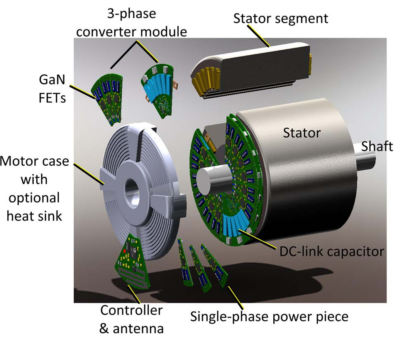
\includegraphics[width=8cm]{images/immd_concept}
  \caption{An IMMD example \cite{Wang2014}}
  \label{fig:immd_concept}
\end{figure}

An IMMD consists of a number of identical modules as shown in Fig. \ref{fig:immd_concept} \cite{Wang2014}. Each module is composed of a stator pole with concentrated coil and a drive unit and its controller dedicated to that stator pole. Having this modular structure with multiple modules brings flexibility to the designer regarding the connection of the motor drive modules on the DC link. In addition, several techniques such as interleaving can be applied for ripple and harmonic component minimization. However, all the methods developed so far are related to the switching frequency. There have been several studies in the literature for the minimization of switching frequency components on the DC link to enhance the power density of the DC link capacitors, however none of them include the effect of 6\textsuperscript{th} harmonic component due to the rectifier. In Dc link capacitor optimization studies, the effect of rectifier harmonics are neglected, and the input side is treated as an ideal DC source, which is not the case in practice.

In this research work, the modular structure is utilized with low order harmonic injection for the cancellation of the 6\textsuperscript{th} harmonic component on the DC link. First, the frequency components are modeled analytically and it is shown that a zero sequence 3\textsuperscript{th} harmonic injection by the motor drive inverters can generate a 6\textsuperscript{th} harmonic component while 2\textsuperscript{nd} and 4\textsuperscript{th} harmonic components are cancelled with a balanced three-phase inverter topology. Then, a mathematical model for the rectifier and DC link LC filter is obtained. These analytical models are verified by simulations carried out in MATLAB/Simulink. Finally, it is shown that, a significant reduction on the DC link capacitor can be achieved with this method and it is verified by simulations.

The report is organized as follows: In section 2, a description of the system is presented and the 6\textsuperscript{th} harmonic problem is shown. In section 3, the mathematical model developed for the harmonic components is presented. In section 4, the third harmonic injection method is explained to cancel the sixth harmonic component. In section 5, simulation results are presented and in section 6, general comments on the results are made.


% Burda ref ver

% Motor'a etkilerini incele (future work)
% Possible module sayıları
% Possible motor bağlantıları



\chapter{Problem Definition}
\label{chap:problem-definition}

A conventional motor drive application block diagram is shown in Fig. \ref{fig:conv_motor_drive}. The DC link decouples the inverter and rectifier such that, its characteristics is effected from both sides. Most studies consider only one side for DC link characterisation or filter component optimization, although they should be considered simultaneously. This research aims at modeling the system as a whole, investigating the effect of harmonic components injected to the DC link from both sides and eliminating the low frequency harmonic due to the rectifier side by using the modular structure of the inverter side.

\begin{figure}[htp]
  \centering
  \includegraphics[width=15cm]{images/conv_motor_drive}
  \caption{A conventional motor drive block diagram}
  \label{fig:conv_motor_drive}
\end{figure}

Diode bridge rectifier is a natural-commutated converter, circuit schematic of which is shown in Fig. \ref{fig:rect_circuit}.

\begin{figure}[htp]
  \centering
  \includegraphics[width=15cm]{images/rect_circuit}
  \caption{Diode bridge rectifier circuit diagram}
  \label{fig:rect_circuit}
\end{figure}

A set of voltage and current waveforms are also shown in Fig. \ref{fig:rect_waveform}, for 400V line-to-line grid voltage at 50 Hz, filter inductance of 1 mH, filter capacitance of 3 mF and load resistance of 
10 $\Omega$. The three-phase rectifier output voltage and current has large harmonic components frequency of which is six times the grid frequency. This component is filtered by a second order LC filter resulting in a much smoother load voltage and current. Since the harmonic frequency is relatively low in comparison with conventional switching frequencies, large inductance and capacitance values are needed on the DC link filter. Those passive elements constitute a large portion of overall volume and cost, hence it is aimed to minimize their values.

\begin{figure}[htp]
  \centering
  \includegraphics[width=15cm]{images/rect_waveform}
  \caption{Diode bridge rectifier input and output waveforms}
  \label{fig:rect_waveform}
\end{figure}






% \begin{figure}[htp]
%   \centering
%   \tikzstyle{block} = [draw, fill=blue!20, rectangle, minimum height=3em, minimum width=6em, text width=6em,text centered]
\begin{tikzpicture}[auto, node distance=3.5cm,>=latex']
\shorthandoff{:} % Evite le bug de compilation avec tikz
    % Longueurs et espacement
    \def\longabove{0.2cm}
    \def\espacement{4cm}

    % Définition des blocs
    \node [block, node distance=\espacement] (codeur) {Codeur};
    \node [block, right of=codeur, node distance=\espacement] (cbs) {CBS};
    \node [block, right of=cbs, node distance=\espacement] (modulateur) {Modulateur};
 
    % Définition des liens
    \draw [<-] (codeur) -- ++(-2,0) node[left] {$\{b_n\}$};
    \draw [->] (codeur) -- node[above=\longabove] {$\{d_n\}$} (cbs);
    \draw [->] (cbs) -- node[above=\longabove] {$\{c_k\}$} (modulateur);
    \draw [->] (modulateur) -- ++(2,0) node[right] {$s(t)$};
\end{tikzpicture}

%   \caption{Exemple de diagramme TikZ.}
%   \label{fig:une-image}
% \end{figure}

% \section{Une autre section}
% Lorem (tab. \ref{tab:un-tableau}).

% \begin{table}[ht]
%   \begin{center}
%     \begin{tabular}{|c|c|c|c|c|}
%       \hline
%       & $h(t,\tau)$ & $S_{\OP{H}}^{(\alpha)} (f,\tau)$ & $L_{\OP{H}}^{(\alpha)} (\nu,t)$ & $H^{(\alpha)}(f,\nu)$ \\
%       \hline
%       LTI & $q(\tau)$ & $q(\tau) \delta(f)$ & $Q(\nu)$ & $Q(\nu) \delta(\nu-f)$ \\
%       \hline
%       LFI & $m(t) \delta(\tau)$ & $M(f) \delta(\tau)$ & $m(t)$ & $M(f)$\\
%       \hline
%       identité & $\delta(t)$ & $\delta(f)\delta(\tau)$ & $1$ & $\delta(\nu-f)$\\
%       \hline
%     \end{tabular}
%     \caption{Exemple de tableau.}
%     \label{tab:un-tableau}
%   \end{center}
% \end{table}


% % \section{Une section}
% % Lorem 


\chapter{System Modeling}
\label{chap:system-modeling}

\section{Diode Bridge Rectifier}
Diode bridge rectifier is a natural-commutated converter, circuit schematic of which is shown in Fig. \ref{fig:rect_circuit}.

\section{Motor Drive Inverter}

\chapter{Description of the Method}
\addcontentsline{chapter}{Description of the Method}

Voltages and current expressions of one inverter module with zero sequence third harmonic injection are shown in \ref{eq:1}-\ref{eq:6}.

\begin{equation} \label{eq:1}
v_a(t) = V_1sin(2\pi ft-\phi_{1v})+V_3sin(6\pi ft-\phi_{3v})
\end{equation}
\begin{equation} \label{eq:2}
v_b(t) = V_1sin(2\pi ft-2\pi/3-\phi_{1v})+V_3sin(6\pi ft-\phi_{3v})
\end{equation}
\begin{equation} \label{eq:3}
v_c(t) = V_1sin(2\pi ft-4\pi/3-\phi_{1v})+V_3sin(6\pi ft-\phi_{3v})
\end{equation}

\begin{equation} \label{eq:4}
i_a(t) = I_1sin(2\pi ft-\phi_{1i})+I_3sin(6\pi ft-\phi_{3i})
\end{equation}
\begin{equation} \label{eq:5}
i_b(t) = I_1sin(2\pi ft-2\pi/3-\phi_{1i})+I_3sin(6\pi ft-\phi_{3i})
\end{equation}
\begin{equation} \label{eq:6}
i_c(t) = I_1sin(2\pi ft-4\pi/3-\phi_{1i})+I_3sin(6\pi ft-\phi_{3i})
\end{equation}

Let us make the definitions shown in \ref{eq:7}-\ref{eq:14}.

\begin{equation} \label{eq:7}
\phi_{11p} = \phi_{1v}+\phi_{1i}
\end{equation}
\begin{equation} \label{eq:8}
\phi_{33p} = \phi_{3v}+\phi_{3i}
\end{equation}
\begin{equation} \label{eq:9}
\phi_{13p} = \phi_{1v}+\phi_{3i}
\end{equation}
\begin{equation} \label{eq:10}
\phi_{31p} = \phi_{3v}+\phi_{1i}
\end{equation}
\begin{equation} \label{eq:11}
\phi_{11n} = \phi_{1v}-\phi_{1i}
\end{equation}
\begin{equation} \label{eq:12}
\phi_{33n} = \phi_{3v}-\phi_{3i}
\end{equation}
\begin{equation} \label{eq:13}
\phi_{13n} = \phi_{1v}-\phi_{3i}
\end{equation}
\begin{equation} \label{eq:14}
\phi_{31n} = \phi_{3v}-\phi_{1i}
\end{equation}

The instantaneous power expression for each phase are shown in \ref{eq:15}-\ref{eq:17}.

\begin{equation}
\label{eq:15}
\begin{multlined}
p_a(t) = 
\frac{V_1I_1}{2} \bigg \lbrack cos(\phi_{11n})-cos(4\pi ft-\phi_{11p}) \bigg \rbrack
+
\frac{V_1I_3}{2} \bigg \lbrack cos(4\pi ft+\phi_{13n})-cos(8\pi ft-\phi_{13p}) \bigg \rbrack
\\
+
\frac{V_3I_1}{2} \bigg \lbrack cos(4\pi ft-\phi_{31n})-cos(8\pi ft-\phi_{31p}) \bigg \rbrack
+
\frac{V_3I_3}{2} \bigg \lbrack cos(\phi_{33n})-cos(12\pi ft-\phi_{33p}) \bigg \rbrack,
\end{multlined}
\end{equation}

\begin{equation}
\label{eq:16}
\begin{multlined}
p_b(t) = 
\frac{V_1I_1}{2} \bigg \lbrack cos(\phi_{11n})-cos(4\pi ft-4\pi/3-\phi_{11p}) \bigg \rbrack
\\
+
\frac{V_1I_3}{2} \bigg \lbrack cos(4\pi ft+ 2\pi/3+\phi_{13n})-cos(8\pi ft-2\pi/3-\phi_{13p}) \bigg \rbrack
\\
+
\frac{V_3I_1}{2} \bigg \lbrack cos(4\pi ft+2\pi/3-\phi_{31n})-cos(8\pi ft-2\pi/3-\phi_{31p}) \bigg \rbrack
\\
+
\frac{V_3I_3}{2} \bigg \lbrack cos(\phi_{33n})-cos(12\pi ft-\phi_{33p}) \bigg \rbrack,
\end{multlined}
\end{equation}

\begin{equation}
\label{eq:17}
\begin{multlined}
p_c(t) = 
\frac{V_1I_1}{2} \bigg \lbrack cos(\phi_{11n})-cos(4\pi ft-8\pi/3-\phi_{11p}) \bigg \rbrack
\\
+
\frac{V_1I_3}{2} \bigg \lbrack cos(4\pi ft+ 4\pi/3+\phi_{13n})-cos(8\pi ft-4\pi/3-\phi_{13p}) \bigg \rbrack
\\
+
\frac{V_3I_1}{2} \bigg \lbrack cos(4\pi ft+4\pi/3-\phi_{31n})-cos(8\pi ft-4\pi/3-\phi_{31p}) \bigg \rbrack
\\
+
\frac{V_3I_3}{2} \bigg \lbrack cos(\phi_{33n})-cos(12\pi ft-\phi_{33p}) \bigg \rbrack,
\end{multlined}
\end{equation}

The total instantaneous power becomes as in \ref{eq:18}. As seen, all the frequency components which are two times and four times the fundamental frequency are cancelled, leaving two DC components and a component at six times the fundamental frequency.

\begin{equation}
\label{eq:18}
\begin{multlined}
p_{total}(t) = 
\frac{V_1I_1}{2} \bigg \lbrack cos(\phi_{11n}) \bigg \rbrack
+
\frac{V_3I_3}{2} \bigg \lbrack cos(\phi_{33n}) \bigg \rbrack
+
\frac{V_3I_3}{2} \bigg \lbrack cos(12\pi ft-\phi_{33p}) \bigg \rbrack
\end{multlined}
\end{equation}


\chapter{Results}
\addcontentsline{chapter}{Results}
\label{chap:results}

    Lorem ipsum dolor sit amet, consectetur adipiscing elit. Sed non risus. Suspendisse lectus tortor, dignissim sit amet, adipiscing nec, ultricies sed, dolor. Cras elementum ultrices diam. Maecenas ligula massa, varius a, semper congue, euismod non, mi. Proin porttitor, orci nec nonummy molestie, enim est eleifend mi, non fermentum diam nisl sit amet erat. Duis semper. Duis arcu massa, scelerisque vitae, consequat in, pretium a, enim. Pellentesque congue. Ut in risus volutpat libero pharetra tempor. Cras vestibulum bibendum augue. Praesent egestas leo in pede. Praesent blandit odio eu enim. Pellentesque sed dui ut augue blandit sodales. Vestibulum ante ipsum primis in faucibus orci luctus et ultrices posuere cubilia Curae; Aliquam nibh. Mauris ac mauris sed pede pellentesque fermentum. Maecenas adipiscing ante non diam sodales hendrerit. Ut velit mauris, egestas sed, gravida nec, ornare ut, mi. Aenean ut orci vel massa suscipit pulvinar. Nulla sollicitudin. Fusce varius, ligula non tempus aliquam, nunc turpis ullamcorper nibh, in tempus sapien eros vitae ligula. Pellentesque rhoncus nunc et augue. Integer id felis. Curabitur aliquet pellentesque diam. Integer quis metus vitae elit lobortis egestas. Lorem ipsum dolor sit amet, consectetuer adipiscing elit. Morbi vel erat non mauris convallis vehicula. Nulla et sapien. Integer tortor tellus, aliquam faucibus, convallis id, congue eu, quam. Mauris ullamcorper felis vitae erat. Proin feugiat, augue non elementum posuere, metus purus iaculis lectus, et tristique ligula justo vitae magna. Aliquam convallis sollicitudin purus. Praesent aliquam, enim at fermentum mollis, ligula massa adipiscing nisl, ac euismod nibh nisl eu lectus. Fusce vulputate sem at sapien. Vivamus leo. Aliquam euismod libero eu enim. Nulla nec felis sed leo placerat imperdiet. Aenean suscipit nulla in justo. Suspendisse cursus rutrum augue. Nulla tincidunt tincidunt mi. Curabitur iaculis, lorem vel rhoncus faucibus, felis magna fermentum augue, et ultricies lacus lorem varius purus. Curabitur eu amet.

%%% Local Variables: 
%%% mode: latex
%%% TeX-master: "isae-report-template"
%%% End: 


\chapter{Conclusions}
\addcontentsline{chapter}{Conclusions}

In this report, a novel method to eliminate the sixth harmonic component on the DC link created by the passive three-phase diode bridge front-end rectifier, by using third harmonic injection in integrated modular motor drive applications.

As a future work, possible motor winding configurations and possible number of inverter modules which can be applied with this method will be studied. The effects of this third harmonic injection method to the motor operation should also be studied and possible counter-measures should be thought. Comparative study should be achieved in terms of inverter performance such as efficiency.



\appendix

% \bibliographystyle{authoryear-fr}
\bibliographystyle{ieeetr}
% \bibliography{references}
\bibliography{IMMDref}


\clearpage

%%%%%%%%%%%%%%%%
%%% Abstract %%%
%%%%%%%%%%%%%%%%

\thispagestyle{empty}

\vspace*{\fill}
\noindent\rule[2pt]{\textwidth}{0.5pt}\\
{\textbf{Résumé ---}}
My name is Mesut Uğur and I a PhD candidate in Electrical and Electronics Engineering Department at Middle East Technical University. I am also working as a Research Assistant in the same department. My main research interests are; power electronics, renewable energy, electric traction systems and embedded hardware system development.

\noindent\rule[2pt]{\textwidth}{0.5pt}
\begin{center}
  METU - EEE\\
  PowerLab
\end{center}
\vspace*{\fill}

\end{document}